\section{Effect of feature correlations}
\label{section:correlations-experiment}

The next experiment aims to analyze how the presence of correlations in data affects the~performance of outlier detection methods. The research is conducted considering various number of features correlated and various correlation strength, under fixed number of training samples and dimension of the feature vectors.


\subsection{Experiment organization}
\label{section:correlations-organization}

The experiment was organized similarly as the one described in the section \ref{section:distributions-organization}.

The difference lies in the definitions of datasets $T$, $K$ and $U$ – utilizing only one generator $G$ – the Multivariate Normal distribution (MVN). The number of training samples was fixed to $n = 2000$, as well as the dimension of feature vectors $d = 1000$. Instead, there are two new parameters introduced:
\vspace{-0.5\baselineskip}
\begin{itemize}
    \item the fraction of features that are correlated $f_{corr}$,
    \item the strength of the features correlation $g_{corr}$ (i.e., covariance value).
\end{itemize}

Both mentioned values affect the content of the covariance matrix $\Sigma$ that is supplied to the MVN generator, e.g., for $d = 8$, $f_{corr} = 0.5$ and $g_{corr} = 0.25$ it would become
\begin{equation}
    \Sigma_{ID}
    =
    \begin{bmatrix}
        \mathbf{1.00} & \mathbf{0.25} & \mathbf{0.25} & \mathbf{0.25} & 0.00 & 0.00 & 0.00 & 0.00 \\
        \mathbf{0.25} & \mathbf{1.00} & \mathbf{0.25} & \mathbf{0.25} & 0.00 & 0.00 & 0.00 & 0.00 \\
        \mathbf{0.25} & \mathbf{0.25} & \mathbf{1.00} & \mathbf{0.25} & 0.00 & 0.00 & 0.00 & 0.00 \\
        \mathbf{0.25} & \mathbf{0.25} & \mathbf{0.25} & \mathbf{1.00} & 0.00 & 0.00 & 0.00 & 0.00 \\
        0.00 & 0.00 & 0.00 & 0.00 & \mathbf{1.00} & 0.00 & 0.00 & 0.00 \\
        0.00 & 0.00 & 0.00 & 0.00 & 0.00 & \mathbf{1.00} & 0.00 & 0.00 \\
        0.00 & 0.00 & 0.00 & 0.00 & 0.00 & 0.00 & \mathbf{1.00} & 0.00 \\
        0.00 & 0.00 & 0.00 & 0.00 & 0.00 & 0.00 & 0.00 & \mathbf{1.00}
    \end{bmatrix}
    .
    \label{eq:corr-example}
\end{equation}

By default the features are not correlated and the variance of all features equals $1.0$.

Only the in-distribution (ID) data (sets $T$ and $K$) are affected by the new parameters. The out-of-distribution (OOD) examples (set $U$) utilizes the identity matrix during generation (i.e., $\Sigma_{OOD} = \mathbb{I}$, features uncorrelated, variance equal to $1.0$).

Summarizing, the input parameters that vary in the experiment are: the fraction of~features that are correlated $f_{corr}$, the strength of the correlation $g_{corr}$, the~distance to~the outliers $h$ and outlierness measure $OF$. The experiment was repeated several times with various values of the generator seed $\xi$.


\subsection{Experiment results}
\label{section:correlations-results}

Second experiment analyzes how the performance of outlierness measures is influenced by the correlations of features in dataset. Surprisingly, there are similarities noticeable when comparing the effect of changed correlation strength for a fixed number of correlated features (figure \ref{fig:covariance}) and the effect of changed fraction of correlated features for a fixed variance (figure \ref{fig:n_correlated}). The experiment involves $n = 2000$ training samples of dimension $d = 1000$ and distance to outliers $h = 8$.

In particular, the ED and SED behave nearly identically in both cases. The correlation of features in data results in more concentrated distribution along a selected direction in the feature space, having an effect similar to the reduction of dimensionality. However, in case of measures that do not consider the correlations, like ED or SED, the result is visible as more extended distribution in space. This effect can be seen in figures \ref{fig:hists-correlations-sed} and \ref{fig:hists-correlations-extreme-sed}. The outcome is worse separability (AUROC value) and classification accuracy for more correlated features, which is caused by the scores for out-of-distribution data appearing within the distribution obtained for training data (especially visible in figure \ref{fig:hists-correlations-extreme-sed}).

The kNN, LOF and MD measures are capable of benefiting from the correlated features, however the nature behind this effect is different. The result in all cases is that the separability of the data is better (greater AUROC values); in general LOF performs slightly better than kNN in this experiment and MD is obtaining the third best separability in most cases for correlated data, i.e., for $f_{corr} > 0.1$ and/or $g_{corr} > 0.1$ (for uncorrelated data, ED and SED performs better than MD here). The effect on AUROC is similar regardless of whether the faction of correlated featured is increased or correlation strength (covariance value) is greater, but for MD the effect is slightly stronger for greater covariance value – i.e., for $g_{corr} \geq 0.4$ it outperforms kNN in the task of separability (and for $g_{corr} \geq 0.5$ it even outperforms LOF). Yet, both kNN and MD are suffering in the task of classification with respect to the training data – due to the same phenomenon already discussed in section \ref{section:distributions-experiment}, i.e., zero sensitivity, all testing in-distribution data are spuriously considered as outliers.

In conducted experiment, only the LOF maintains the good accuracy in the classification task, benefiting from the correlated features. Comparing the figures \ref{fig:hists-correlations-lof} and \ref{fig:hists-correlations-extreme-lof}, it is because out-of-distribution data are seen as more distant in case of stronger correlation in the in-distribution dataset.

Interesting observation can be made when comparing figures \ref{fig:hists-correlations-knn} and \ref{fig:hists-correlations-extreme-knn} (kNN) with figures \ref{fig:hists-correlations-md} and \ref{fig:hists-correlations-extreme-md} (MD). In both cases the better separation between in-distribution test data and out-of-distribution samples is visible for more correlated features. However, in case of kNN, the effect of data concentration is visible – obtained score values for training data and known examples (clusters $T$ and $K$) are lower, corresponding with smaller spatial distances. Contrary, in case of MD, scores for both in-distribution data do not change significantly, yet still the outliers (cluster $U$) appears noticeably farther distanced.

\begin{figure}[t]
    \centering
    \begin{subfigure}[b]{0.9\textwidth}
        % StreamLit settings: width=9, height=4
        % X: [-0.01, 1.01]
        % Y: [0.69, 1.01]
        \centering
        \caption{\small Separability between in-distribution and out-of-distribution data}
        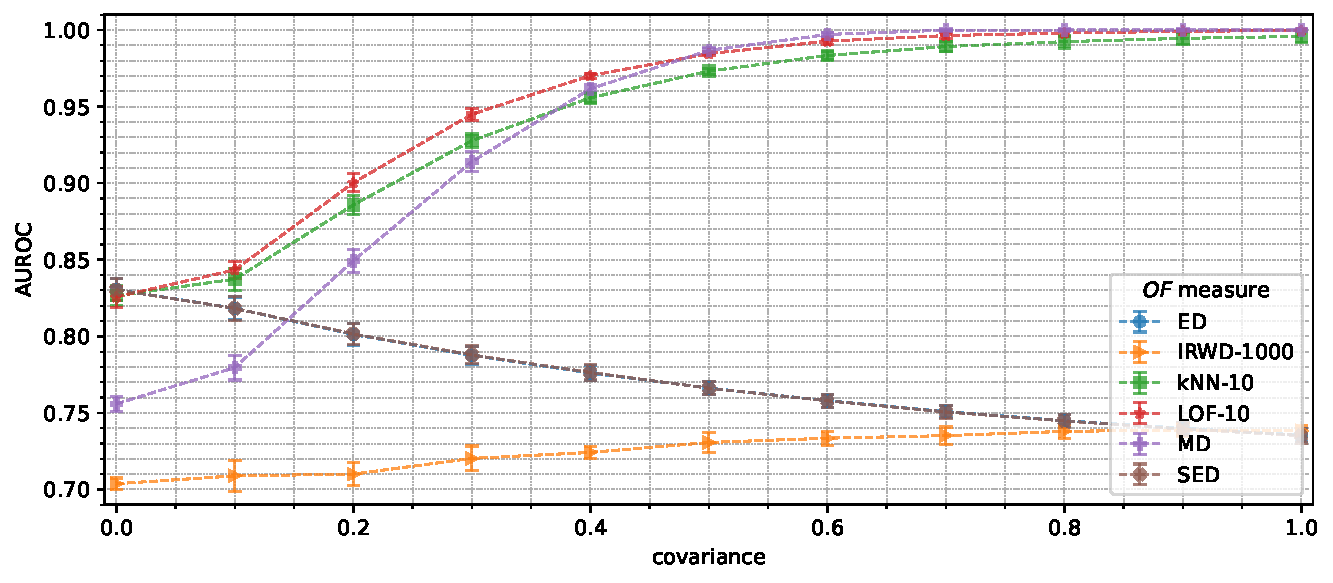
\includegraphics[width=\textwidth]{images/correlations/g_corr/trend-correlations-auroc(covariance)-n_correlated_0.20-distance_8-outliers_correlated_False-model_ED,IRWD-1000,kNN-10,LOF-10,MD,SED-aggregated.pdf}
        \label{fig:covariance-auroc}
    \end{subfigure}
    \begin{subfigure}[b]{0.9\textwidth}
        % StreamLit settings: width=9, height=4
        % X: [-0.01, 1.01]
        % Y: [0.44, 1.00]
        \centering
        \caption{\small Classification with respect to the training data}
        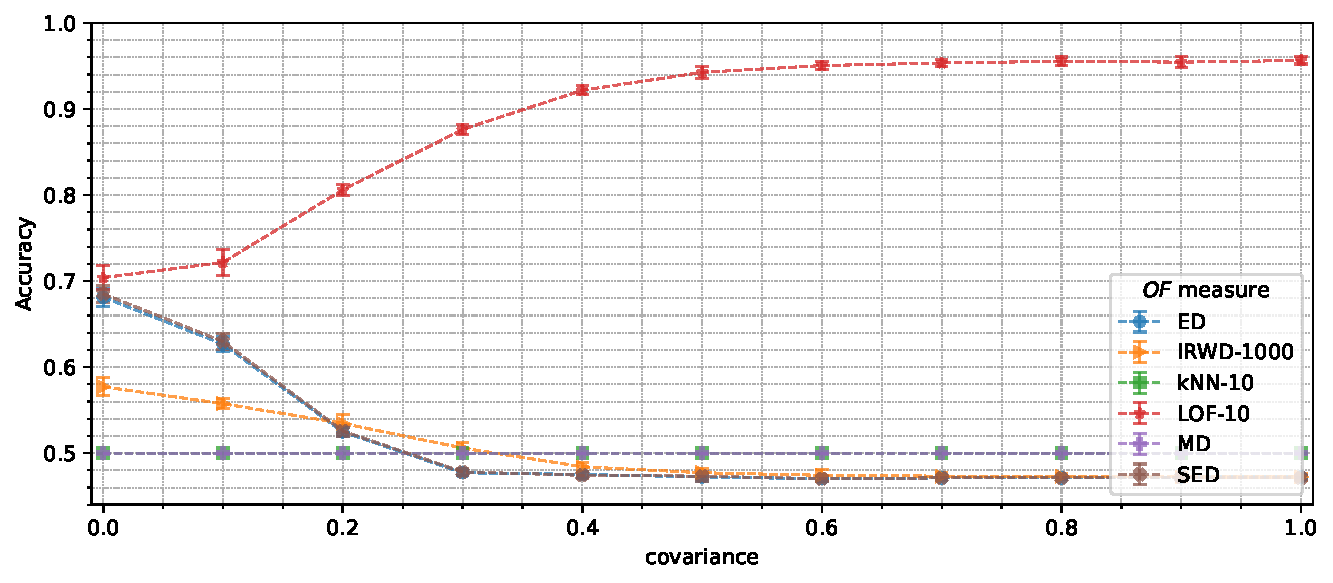
\includegraphics[width=\textwidth]{images/correlations/g_corr/trend-correlations-accuracy_95(covariance)-n_correlated_0.20-distance_8-outliers_correlated_False-model_ED,IRWD-1000,kNN-10,LOF-10,MD,SED-agg.pdf}
        \label{fig:covariance-accuracy}
    \end{subfigure}
    \begin{subfigure}[b]{0.495\textwidth}
        % StreamLit settings: width=5, height=3
        % X: [-0.01, 1.01]
        % Y: [-0.02, 1.05]
        \centering
        \caption{\small Correctly recognized in-distribution}
        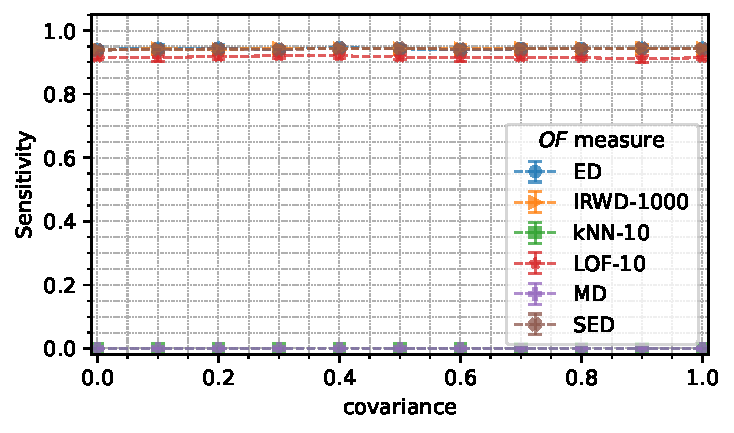
\includegraphics[width=\textwidth]{images/correlations/g_corr/trend-correlations-sens_95(covariance)-n_correlated_0.20-distance_8-outliers_correlated_False-model_ED,IRWD-1000,kNN-10,LOF-10,MD,SED-aggregated.pdf}
        \label{fig:covariance-sensitivity}
    \end{subfigure}
    \hfill
    \begin{subfigure}[b]{0.495\textwidth}
        % StreamLit settings: width=5, height=3
        % X: [-0.01, 1.01]
        % Y: [-0.02, 1.05]
        \centering
        \caption{\small Correctly recognized out-of-distribution}
        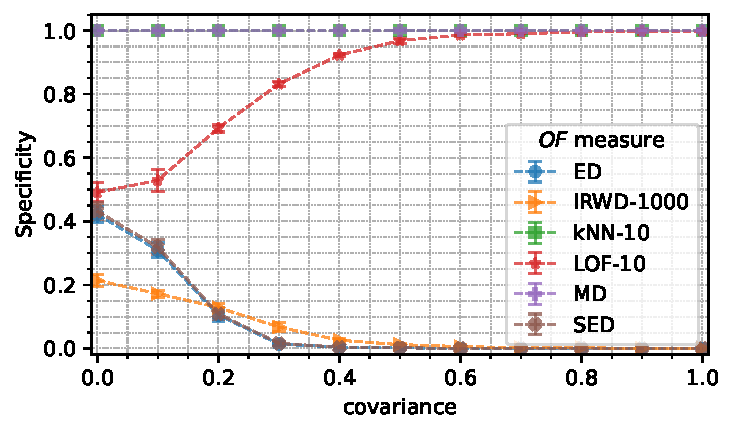
\includegraphics[width=\textwidth]{images/correlations/g_corr/trend-correlations-spec_95(covariance)-n_correlated_0.20-distance_8-outliers_correlated_False-model_ED,IRWD-1000,kNN-10,LOF-10,MD,SED-aggregated.pdf}
        \label{fig:covariance-specificity}
    \end{subfigure}
    \caption{The performance of outlierness measures $OF$ as affected by the correlation strength (covariance value $g_{corr}$). The fixed parameters in the experiment are: dimension of the~feature space $d = 1000$, number of training samples $n = 2000$, distance to outliers $h = 8$ and fraction of features that are correlated $f_{corr} = 0.2$. The~results are aggregated for multiple generator seeds $\xi$ and displayed as averages with~error~bars (standard deviation).}
    \label{fig:covariance}
    \vspace{-2.3em}
\end{figure}

\begin{figure}[t]
    \centering
    \begin{subfigure}[b]{0.9\textwidth}
        % StreamLit settings: width=9, height=4
        % X: [-0.01, 1.01]
        % Y: [0.69, 1.01]
        \centering
        \caption{\small Separability between in-distribution and out-of-distribution data}
        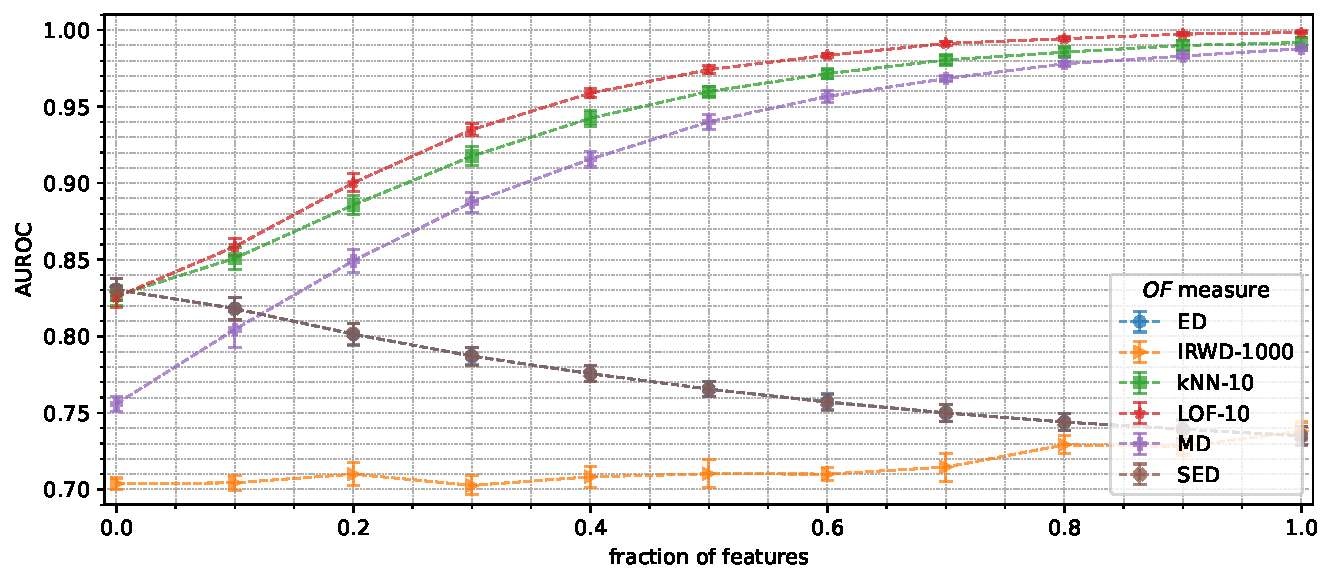
\includegraphics[width=\textwidth]{images/correlations/f_corr/trend-correlations-auroc(n_correlated)-covariance_0.20-distance_8-outliers_correlated_False-model_ED,IRWD-1000,kNN-10,LOF-10,MD,SED-aggregated.pdf}
        \label{fig:n_correlated-auroc}
    \end{subfigure}
    \begin{subfigure}[b]{0.9\textwidth}
        % StreamLit settings: width=9, height=4
        % X: [-0.01, 1.01]
        % Y: [0.44, 1.00]
        \centering
        \caption{\small Classification with respect to the training data}
        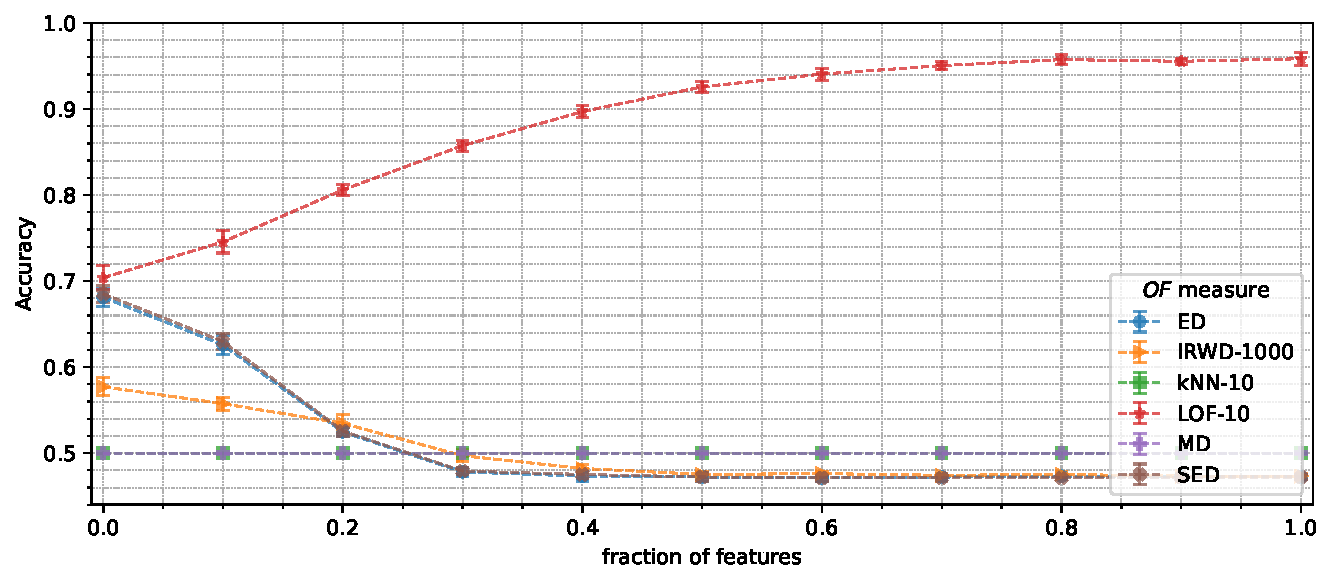
\includegraphics[width=\textwidth]{images/correlations/f_corr/trend-correlations-accuracy_95(n_correlated)-covariance_0.20-distance_8-outliers_correlated_False-model_ED,IRWD-1000,kNN-10,LOF-10,MD,SED-agg.pdf}
        \label{fig:n_correlated-accuracy}
    \end{subfigure}
    \begin{subfigure}[b]{0.495\textwidth}
        % StreamLit settings: width=5, height=3
        % X: [-0.01, 1.01]
        % Y: [-0.02, 1.05]
        \centering
        \caption{\small Correctly recognized in-distribution}
        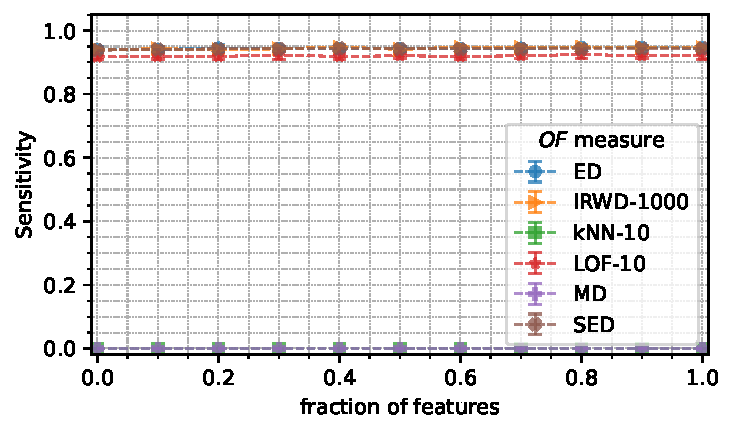
\includegraphics[width=\textwidth]{images/correlations/f_corr/trend-correlations-sens_95(n_correlated)-covariance_0.20-distance_8-outliers_correlated_False-model_ED,IRWD-1000,kNN-10,LOF-10,MD,SED-aggregated.pdf}
        \label{fig:n_correlated-sensitivity}
    \end{subfigure}
    \hfill
    \begin{subfigure}[b]{0.495\textwidth}
        % StreamLit settings: width=5, height=3
        % X: [-0.01, 1.01]
        % Y: [-0.02, 1.05]
        \centering
        \caption{\small Correctly recognized out-of-distribution}
        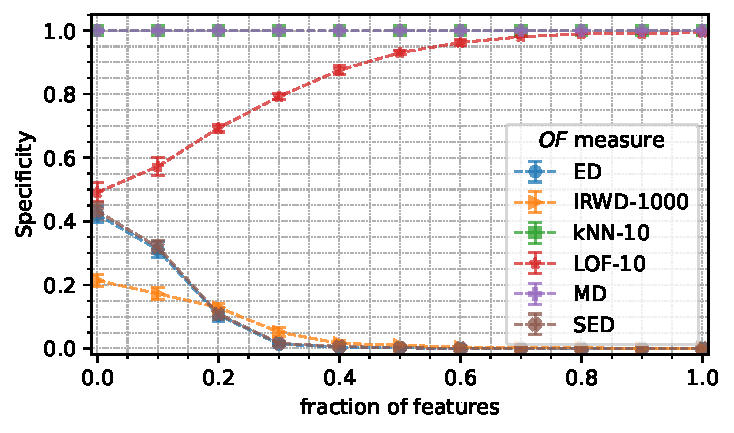
\includegraphics[width=\textwidth]{images/correlations/f_corr/trend-correlations-spec_95(n_correlated)-covariance_0.20-distance_8-outliers_correlated_False-model_ED,IRWD-1000,kNN-10,LOF-10,MD,SED-aggregated.pdf}
        \label{fig:n_correlated-specificity}
    \end{subfigure}
    \caption{The performance of outlierness measures $OF$ as affected by the fraction of features that are correlated $f_{corr}$. The fixed parameters in the experiment are: dimension of the~feature space $d = 1000$, number of training samples $n = 2000$, distance to outliers $h = 8$ and correlation strength (covariance value $g_{corr} = 0.2$). The~results are aggregated for multiple generator seeds $\xi$ and displayed as averages with~error~bars~(standard deviation).}
    \label{fig:n_correlated}
    \vspace{-2.3em}
\end{figure}

\begin{figure}[t]
    % StreamLit settings: width=9, height=2
    \centering
    \begin{subfigure}[b]{\textwidth}
        \centering
        \caption{\small k-Nearest Neighbors ($k=10$), covariance: $g_{corr} = 0.2$, fraction: $f_{corr} = 0.2$}
        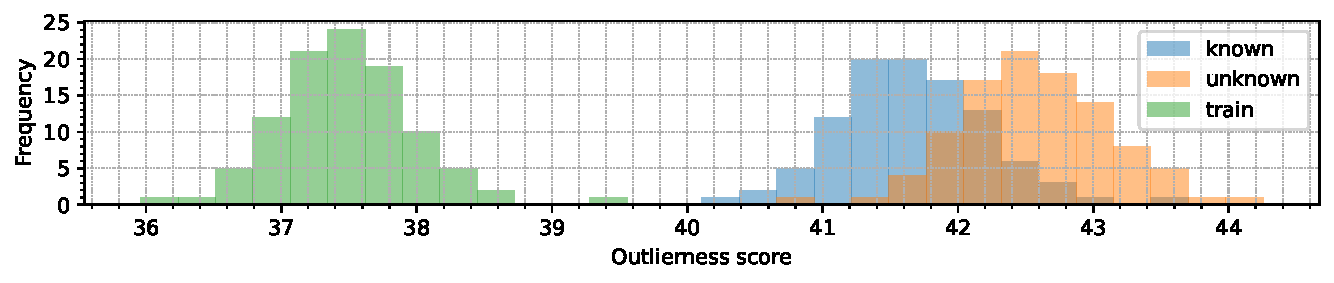
\includegraphics[width=\textwidth]{images/correlations/hists/hist-correlations-n_correlated_0.20-covariance_0.20-distance_8-outliers_correlated_False-model_kNN-10-seed_0.pdf}
        \label{fig:hists-correlations-knn}
    \end{subfigure}
    \begin{subfigure}[b]{\textwidth}
        \centering
        \caption{\small Local Outlier Factor ($k=10$), covariance: $g_{corr} = 0.2$, fraction: $f_{corr} = 0.2$}
        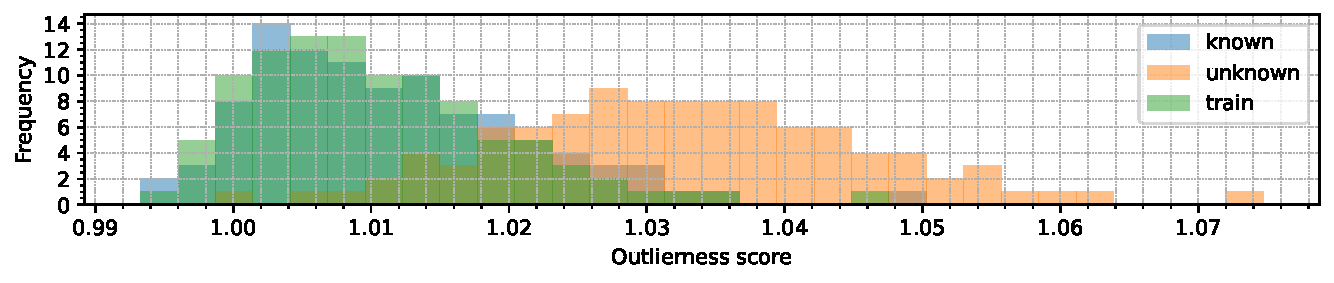
\includegraphics[width=\textwidth]{images/correlations/hists/hist-correlations-n_correlated_0.20-covariance_0.20-distance_8-outliers_correlated_False-model_LOF-10-seed_0.pdf}
        \label{fig:hists-correlations-lof}
    \end{subfigure}
    \begin{subfigure}[b]{\textwidth}
        \centering
        \caption{\small Mahalanobis distance, covariance: $g_{corr} = 0.2$, fraction: $f_{corr} = 0.2$}
        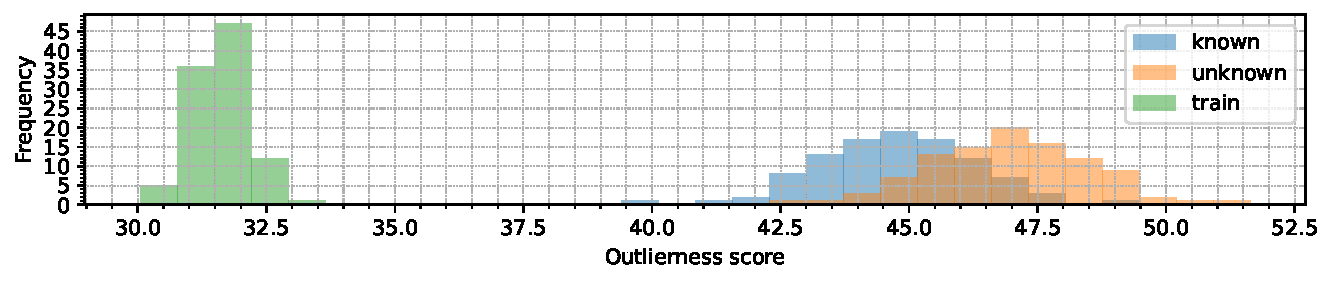
\includegraphics[width=\textwidth]{images/correlations/hists/hist-correlations-n_correlated_0.20-covariance_0.20-distance_8-outliers_correlated_False-model_MD-seed_0.pdf}
        \label{fig:hists-correlations-md}
    \end{subfigure}
    \begin{subfigure}[b]{\textwidth}
        \centering
        \caption{\small Standardized Euclidean distance, covariance: $g_{corr} = 0.2$, fraction: $f_{corr} = 0.2$}
        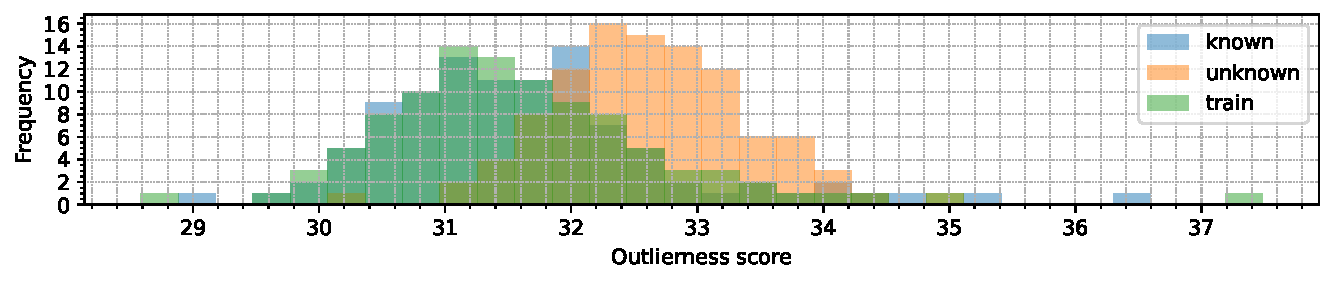
\includegraphics[width=\textwidth]{images/correlations/hists/hist-correlations-n_correlated_0.20-covariance_0.20-distance_8-outliers_correlated_False-model_SED-seed_0.pdf}
        \label{fig:hists-correlations-sed}
    \end{subfigure}
    \caption{Distributions of outlierness scores for various measures $OF$ with a~small fraction of features slightly correlated. The correlation makes the generated clusters more concentrated in space, resulting in a better separability in case of kNN, LOF and~MD, except for SED that is not considering correlations (compare with figure \ref{fig:hists-correlations-extreme}). Other experiment parameters involved: dimension of feature space $d = 1000$, number of~training samples $n = 2000$, distance~to~outliers $h = 8$, generator seed $\xi = 0$.}
    \label{fig:hists-correlations}
\end{figure}

\begin{figure}[t]
    % StreamLit settings: width=9, height=2
    \centering
    \begin{subfigure}[b]{\textwidth}
        \centering
        \caption{\small k-Nearest Neighbors ($k=10$), covariance: $g_{corr} = 0.5$, fraction: $f_{corr} = 0.5$}
        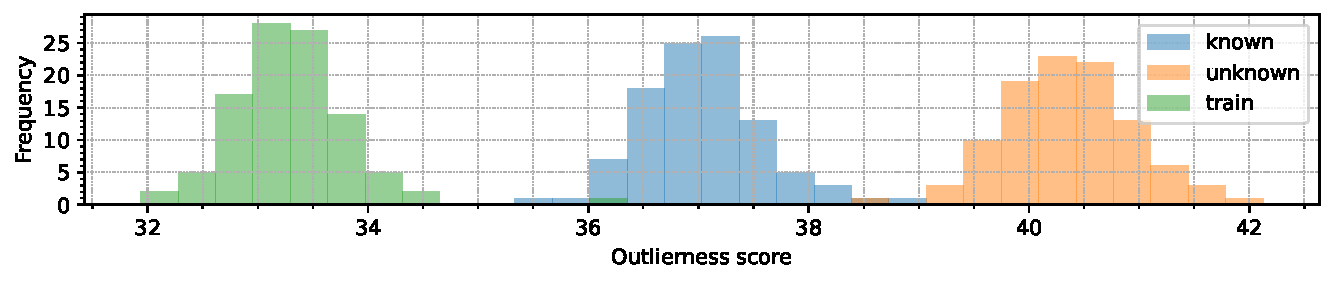
\includegraphics[width=\textwidth]{images/correlations/hists-extreme/hist-correlations-n_correlated_0.50-covariance_0.50-distance_8-outliers_correlated_False-model_kNN-10-seed_0.pdf}
        \label{fig:hists-correlations-extreme-knn}
    \end{subfigure}
    \begin{subfigure}[b]{\textwidth}
        \centering
        \caption{\small Local Outlier Factor ($k=10$), covariance: $g_{corr} = 0.5$, fraction: $f_{corr} = 0.5$}
        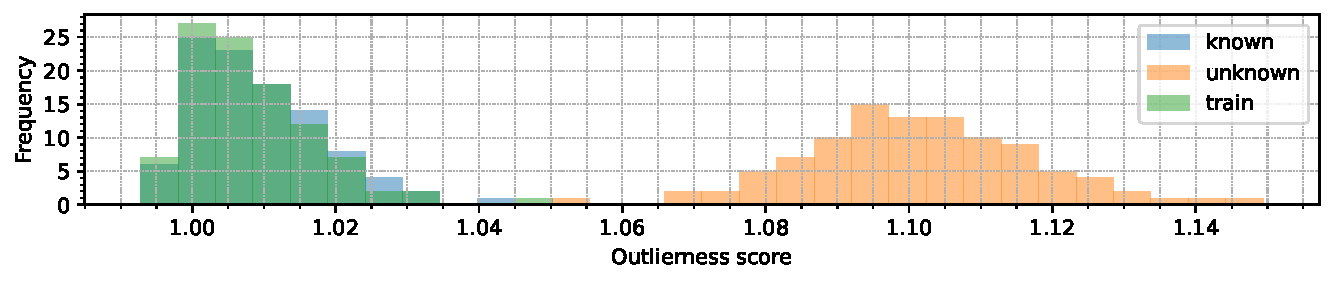
\includegraphics[width=\textwidth]{images/correlations/hists-extreme/hist-correlations-n_correlated_0.50-covariance_0.50-distance_8-outliers_correlated_False-model_LOF-10-seed_0.pdf}
        \label{fig:hists-correlations-extreme-lof}
    \end{subfigure}
    \begin{subfigure}[b]{\textwidth}
        \centering
        \caption{\small Mahalanobis distance, covariance: $g_{corr} = 0.5$, fraction: $f_{corr} = 0.5$}
        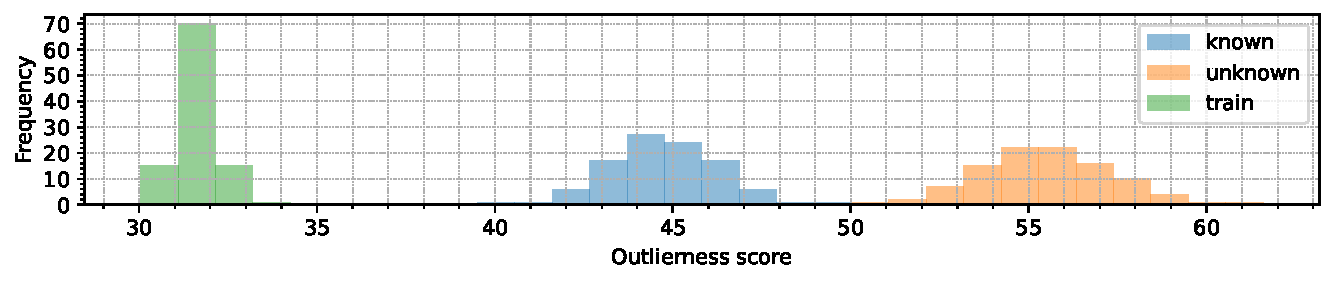
\includegraphics[width=\textwidth]{images/correlations/hists-extreme/hist-correlations-n_correlated_0.50-covariance_0.50-distance_8-outliers_correlated_False-model_MD-seed_0.pdf}
        \label{fig:hists-correlations-extreme-md}
    \end{subfigure}
    \begin{subfigure}[b]{\textwidth}
        \centering
        \caption{\small Standardized Euclidean distance, covariance: $g_{corr} = 0.5$, fraction: $f_{corr} = 0.5$}
        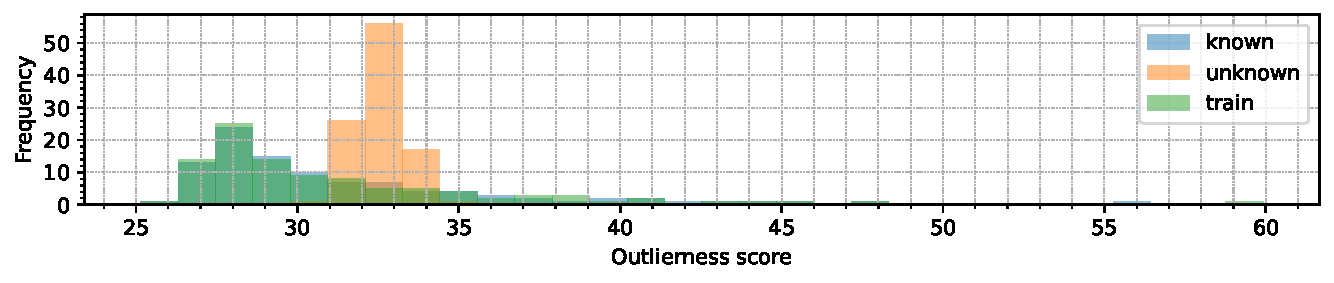
\includegraphics[width=\textwidth]{images/correlations/hists-extreme/hist-correlations-n_correlated_0.50-covariance_0.50-distance_8-outliers_correlated_False-model_SED-seed_0.pdf}
        \label{fig:hists-correlations-extreme-sed}
    \end{subfigure}
    \caption{Distributions of outlierness scores for various measures $OF$ with a~half of~features highly correlated. The significant correlation results in much~better separability in case of kNN, LOF and~MD; in case of not considering correlations SED measure, a long right tail appears (compare with figure \ref{fig:hists-correlations}). Other experiment parameters involved: dimension of feature space $d = 1000$, number of~training samples $n = 2000$, distance~to~outliers $h = 8$, generator seed $\xi = 0$.}
    \label{fig:hists-correlations-extreme}
\end{figure}

\cleardoublepage{}
